\section{How Does It Work?}
\label{sec:functionality}

In UAS, there are three types of entities: issuers, users, and openers. However,
cryptographically speaking, users and issuers are the same, with the only
exception that issuers advertise their public keys, and policy for issuance.

Users receive credentials from issuers -- a user can own multiple credentials,
even from the same issuer. Then, users leverage (one or more of) these
credentials to produce a signature. As part of producing a signature, users
may need to reveal arbitrary facts related to their credentials and, in
addition, specify an opener. If the need arises, this opener can extract further
information from the signature and involved credentials, in a process that is
known as \emph{opening} a signature. Crucially, no more information than what
the user chooses to reveal can be learned from the signature; yet, the verifier
gets full certainty that the signature comes from a user with a (set of) valid
credential(s). This high-level usage is defined in \figref{fig:functionality}

\begin{figure}[ht!]
  \centering
  % \input{figures/functionality-op.tex}
  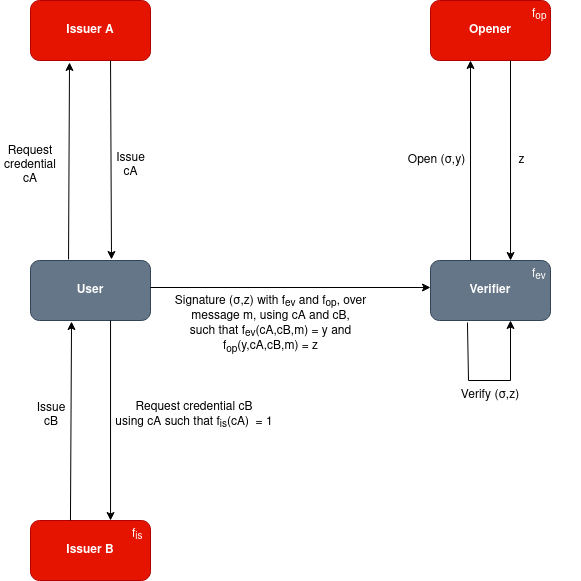
\includegraphics[width=0.8\textwidth]{figures/uas-functionality.png}
  \caption{Sketch of the functionality in UAS schemes, and how the main actors
    interact through this functionality.}
  \label{fig:functionality}
\end{figure}

What makes UAS flexible, though, is the possibility to configure even on a
per-signature basis, the information that will be revelealed, at what time. We
do this via three \emph{functional placeholders}:

\begin{description}
\item[Issuance functions, \fissue:] Issuers are required to specify what
  conditions need to be satisfied by users asking them for credentials. This is
  especially useful when a user wants (or needs) to leverage previously obtained
  credentials (from the same or a different issuer) in order to support its new
  request.
\item[Signature evaluation functions, \feval:] To produce a signature, verifiers
  require that signers prove arbitrary facts over (a subset of) their
  credentials, including revealing specific attributes. This requirement is
  specified, on a per-signature basis, via a signature evaluation function,
  which may also be dependent on the signed message.
\item[Opening functions, \finsp:] On certain scenarios, after a signature is
  produced by its signer, additional information may be required. Opening
  functions control what information can be extracted in such cases, dependent
  on the signer's credentials, the signed message and, also, on the output of
  the evaluation function. In any case, only openers chosen by the signer will
  be able to extract this information.
\end{description}

In a nutshell, UAS provides the general framework for theoretical security and
privacy analysis -- and the $(\fissue,\feval,\finsp)$ functions define the
actual utility-vs-privacy tradeoff that is achieved. Importantly, since these
functions depend on user-private data, they have to be computed by the user.
But, at the same time, issuers, verifiers, and openers need to have certainty
that they have been computed correctly. Thus, zero-knowledge proofs%
\footnote{See, for instance, the Wikipedia entry, for a gentle introduction to
  the topic: \url{https://en.wikipedia.org/wiki/Zero-knowledge_proof}. Last
  access, August 30th, 2022.} play a crucial role in UAS.

%%% Local Variables:
%%% mode: latex
%%% TeX-master: "uas-onepager"
%%% End:
